\section{ПОСТАНОВКА ЗАДАЧИ И ТЕОРЕТИЧЕСКИЕ ПРЕДПОСЫЛКИ}

Итак, перед нами стоит задача разработки прототипа платформы, позволяющей преобразовывать изображение с математическим текстом в \LaTeX-код.

\subsection{Пользовательские сценарии}
Для того, чтобы определить требования к нашей платформе, были проработаны пользовательские сценарии.

Для начала определим основные роли целевых пользователей:
\begin{enumerate}
    \item Пользователь приложения
    \item Программист, использующий $API$ сервиса распознования
\end{enumerate}
Под пользователем приложения подразумевается пользователь одного из типов приложения:
\begin{itemize}
    \item $WEB$ приложение
    \item $Desktop$ приложение
    \item мобильное приложение
\end{itemize}

\subsubsection{Авторизация пользователя}
\underline{Участники:} пользователь любого из типов приложения

\underline{Предусловие:} пользователь запускает приложение впервые или хочет зайти с другого аккаунта

\underline{Постусловие:} пользователь авторизован через $Google$ и предоставлен доступ к $Google\;Drive$

\underline{Сценарий:}
Для авторизации с помощью $Google$ необходимо реализовать следующий сценарий, изображенный на рисунке ~\ref{auth}:

\begin{figure}
    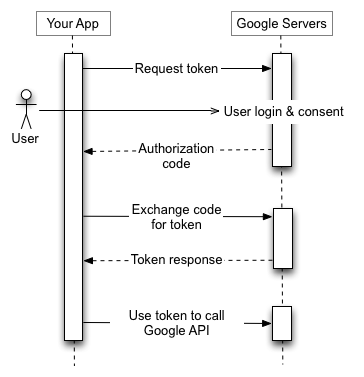
\includegraphics[scale=0.5]{img/use_cases/authorization.png}
    \caption{Сценарий сетевого взаимодействия при авторизациии пользователя}
    \label{auth}
\end{figure}

По сути $Google$ делает всё сам на этапе создания сервиса внутри кода. Если приложение не видит токена для авторизации, то происходит автоматическое перенаправление на сайт авторизации. Дальнейший токен сохраняется локально.

Для замены аккаунта достаточно удалить локальный токен пользователя и перезапустить сервис $Google$. Стоит отметить, что в лучше сохранять токен для дальнейшего быстрого входа в сервис. Но так как мы разрабатываем прототип, то и этого решения будет вполне достаточно.

\subsubsection{Преобразование фотографии}
\underline{Участники:} пользователь приложения

\underline{Предусловие:} пользователь сделал фото научного текста и открыл его в приложении

\underline{Постусловие:} пользователь получает готовый \LaTeX\; код текста, полученного на изображении в виде архива из исходного кода и $pdf$ файла

\underline{Сценарий:}
\begin{enumerate}
    \item Производится автоматическая коррекция перспективы фотографии
    \item Производится автоматическое сегментация текста на абзацы
    \item С приложения на сервер отправляется изображение, а также таблица с координатами начала и конца абзацев
    \item С сервера на приложение отправляется таблица с найденными формулами
    \item Пользователь проверяет правильность распознования формул и вносит коррективы
    \item Приложение отправляет на сервер таблицу с финальными формулами
    \item Сервер загружает архив с \LaTeX\; кодом и $pdf$ файлом в $Google\;Drive$, а также отсылает его пользователю
    \item $Desktop$ приложение обновляет папку $Google\;Drive$ и загружает в локальное хранилище последний архив
\end{enumerate}

При необходимости пользователь может корректировать точки перспективы, а также точки абзацев на изображении.

\subsubsection{Преобразование скриншота}
\underline{Участники:} пользователь приложения

\underline{Предусловие:} пользователь сделал скриншот научного текста и открыл приложение

\underline{Постусловие:} пользователь получает готовый \LaTeX\; код текста, полученного на изображении в виде архива из исходного кода и $pdf$ файла

\underline{Сценарий:} да вроде такой же сценарий, ничем не отличается...

\subsection{Метрики}
Ну тут стандартные, когда-нибудь будет что-то и про них...